\begin{figure}[t]
  \scalebox{0.92}{
    \begin{tabular}{m{1pt}c@{\hspace{10pt}}c@{\hspace{10pt}}c}
      &\hspace{7pt}\small model: \labelcref{item:many-neuron-model}; data: $\texttt{Kur}(10)$) &
      \hspace{7pt}\small model: \labelcref{item:many-neuron-model}; data: $\texttt{Kur}(4)$ &
      \hspace{7pt}\small model: ICA; data: $\texttt{Kur}(3)$ \\
      \raisebox{62pt}{\rotatebox{90}{\tiny magnitude $w_i$}} &
      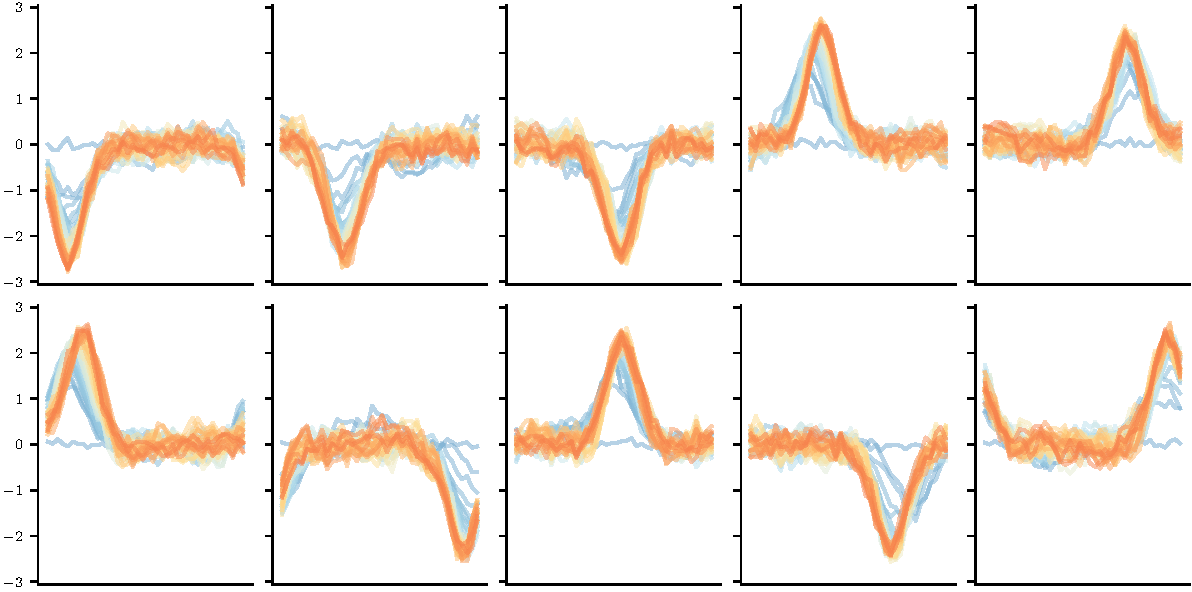
\includegraphics[width=0.33\linewidth]{figures/extensions/10erf_alg10.pdf} &
      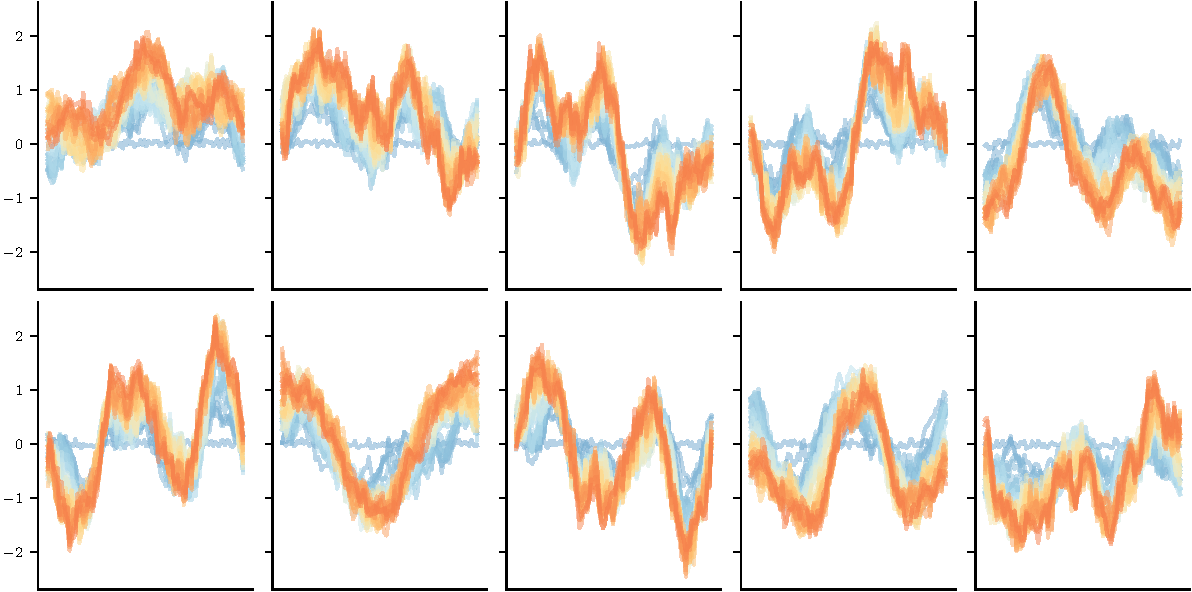
\includegraphics[width=0.33\linewidth]{figures/extensions/10erf_alg4.pdf} &
      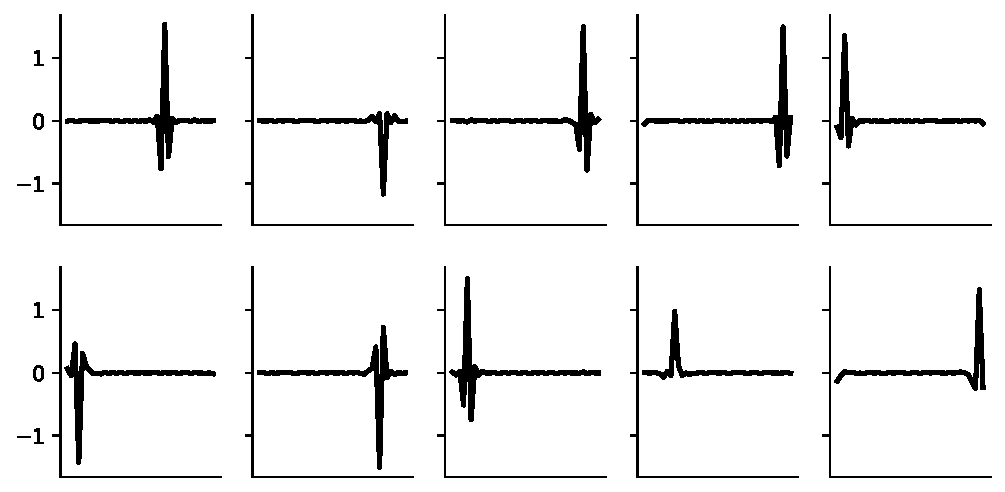
\includegraphics[width=0.33\linewidth]
      {figures/extensions/ica_alg3.pdf} \\
    \noalign{\vskip -48pt}
      &\hspace{7pt}\tiny dimension $i$ of weight $\mathbf{w}$ &
      \hspace{7pt}\tiny dimension $i$ of weight $\mathbf{w}$ &
    \hspace{7pt}\tiny dimension $i$ of weight $\mathbf{w}$
    \end{tabular}
  }
  \caption{
    (\textbf{左}, \textbf{中}) 由多神经元(\labelcref{item:many-neuron-model})软委员会机器(第二层权重固定为 $\frac{1}{K}$)学习到的感受野,分别在 $\texttt{Kur}(10)$ 和 $\texttt{Kur}(4)$ 数据集上训练得到。
    模型具有 $N=40$ 个输入单元,$K=10$ 个隐藏单元,初始化方差为 $0.1$。
    (\textbf{右}) 从 scikit-learn 的 FastICA 算法中学习到的 40 个分量的随机子集,其中包含 10 个分量,使用的 $\texttt{Kur}(3)$ 数据集,其长度尺度相关值为 $\xi_0 = 1$ 和 $\xi_1 = 3$。
    \emph{参见 \cref{sec:extensions} 以了解详细说明。}
}
  \label{fig:extensions}
\end{figure}
